\documentclass[11pt,a4paper]{article}

\usepackage{amsmath} %for mathemathic formulas
\usepackage{amssymb}
\usepackage[ngerman]{babel} %for the german language by the spellling reform (without the package the date would look like April 20, 2020)
\usepackage{enumitem} %for enumeration surrounding
\usepackage{graphicx} %for pictures
\usepackage{siunitx}

\title{Blatt 4}
\date{\today}
\author{Hannah Rotgeri \and Lena Olbrich}

\begin{document}
    \maketitle

    \section*{Aufgabe 1}
\subsection*{Aufgabenteil a}
Zuerst Nummierung berechnen :
\begin{align*}
1= \int_{-\pi}^{\pi} N e^{-|\psi| k} d\psi= N \left( [\frac{1}{k}e^{\psi k}]^0_{-\pi} + [-\frac{1}{k}e^{-\psi k}]^\pi_{0}\right)=\frac{2}{k}(1-e^{-\pi k}) \Leftrightarrow N=\frac{k}{2(1-e^{-\pi k})}
\end{align*}
Wurde implemetiert, aber leider nicht erfolgreich getestet

\subsection*{Aufgabenteil b}
Kumulative Verteilung berechnen:
\begin{align*}
A(x)=\int_{-\pi}^{\psi}e^{-|\psi|k}d\psi=
\int_{-\pi}^{0} e^{\psi k} d \psi + \int_{0}^{\psi} e^{-\psi k} d \psi \\
= \left[\frac{1}{k} e^{\psi k}\right]^0_{-\pi} +\left[-\frac{1}{k}e^{-\psi k}\right]^\psi_0
=\frac{1}{k}\left(2- e^{-\pi k} - e^{-\psi k} \right)
\end{align*}
Normierte Fläche:
\begin{align*}
r(x)= A(x)\cdot N = \left(2- e^{-\pi k} - e^{-\psi k} \right) \cdot \frac{1}{2(1-e^{-\pi k})}
\end{align*}
Wurde implemetiert, aber nicht erfolgreich getestet
\subsection*{Aufgabenteil c}
Inverse berechnen:
\begin{align*}
 \psi(r)=-\frac{1}{k}\ln(2-2r(1-e^{-\pi k})-e^{-\pi k})
\end{align*}
Wurde implemetiert, aber nicht erfolgreich getestet

\begin{figure}[h]

	\centering

	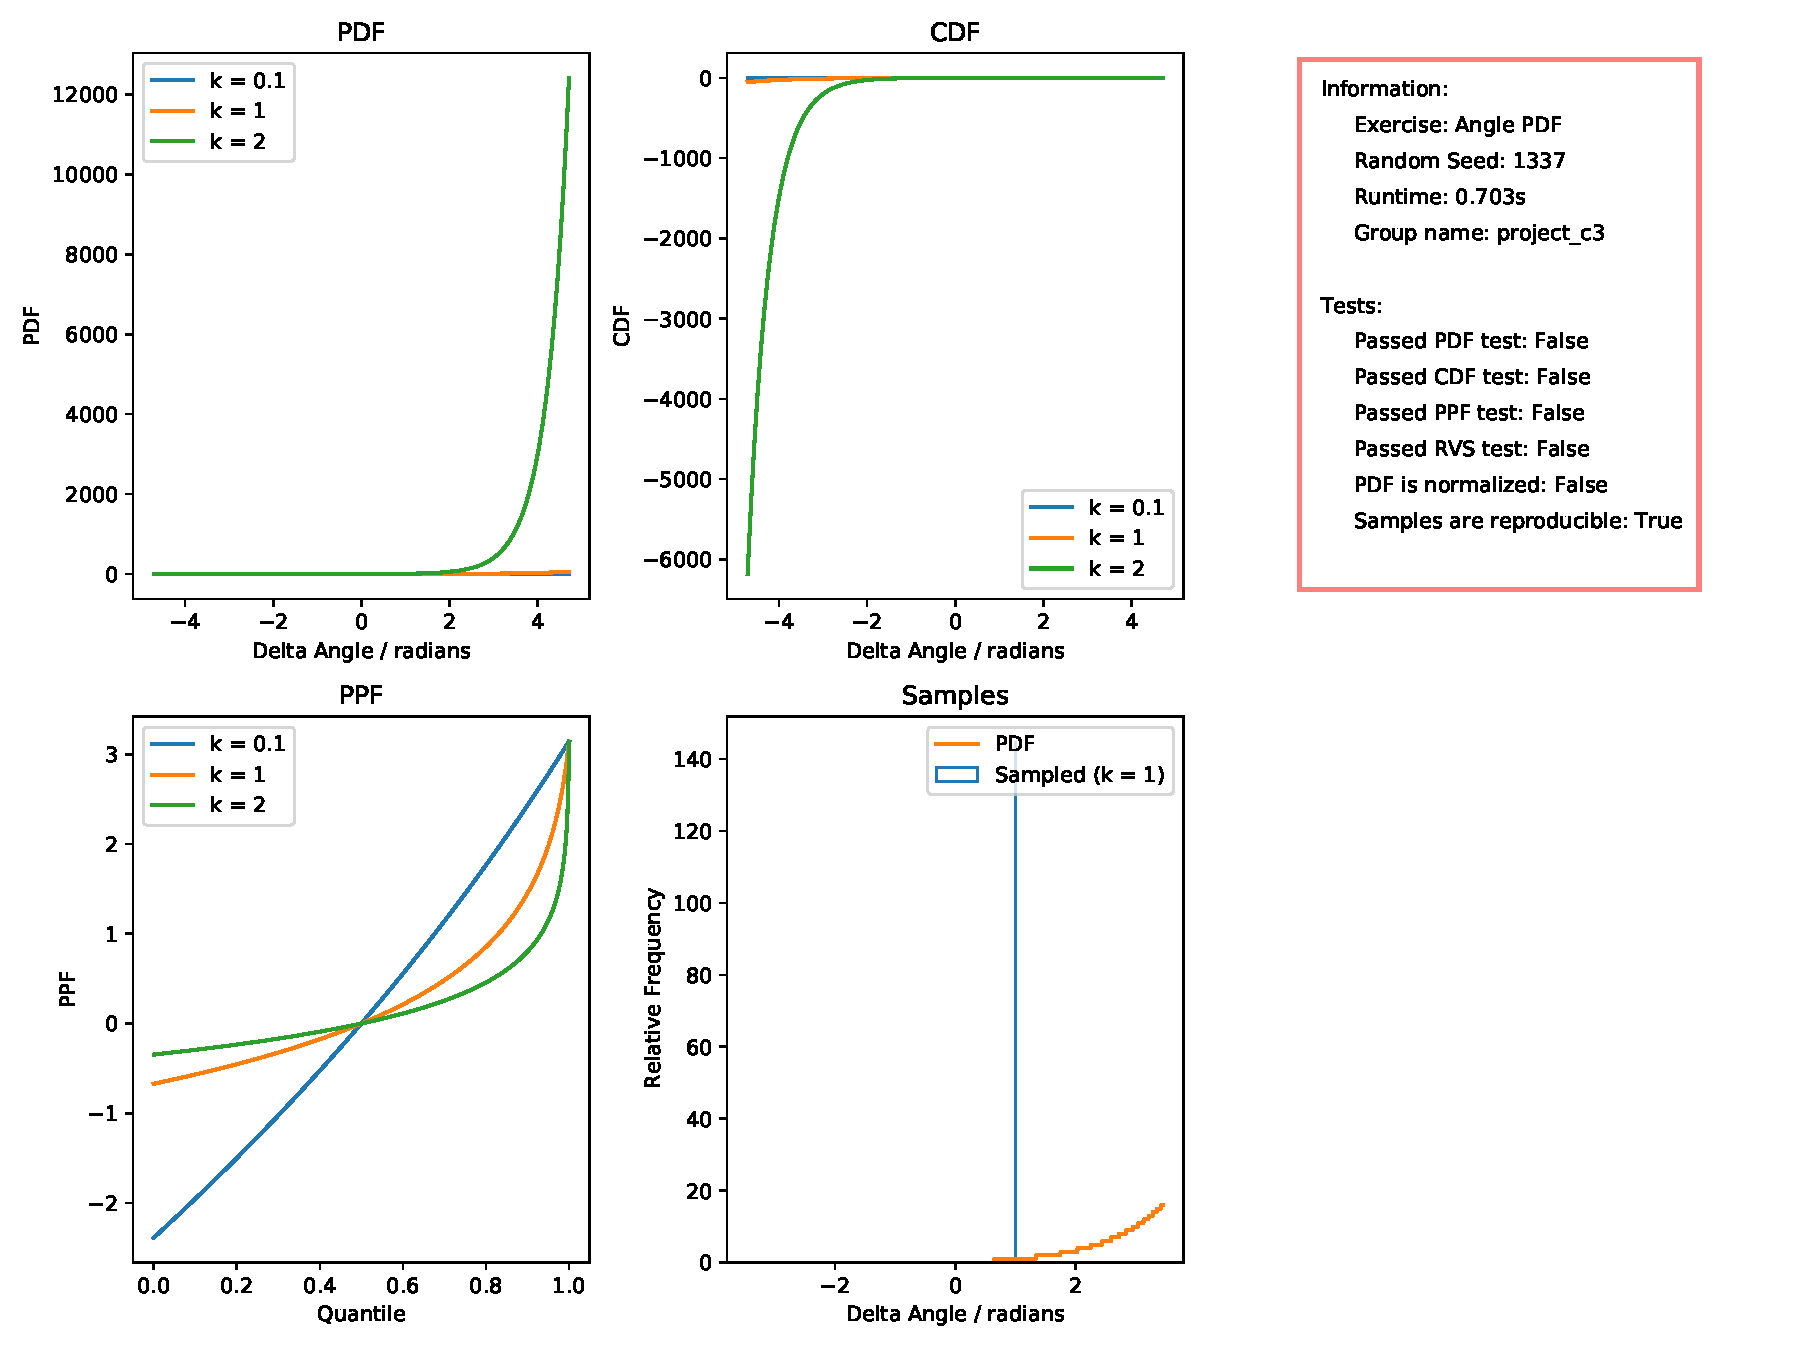
\includegraphics[width=\textwidth]{exercise_angle_pdf.pdf}

	\caption{Ergebnis der Testdatei von Aufgabe 1}

\end{figure}

\section*{Aufgabe 2}

\begin{figure}[h]

	\centering

	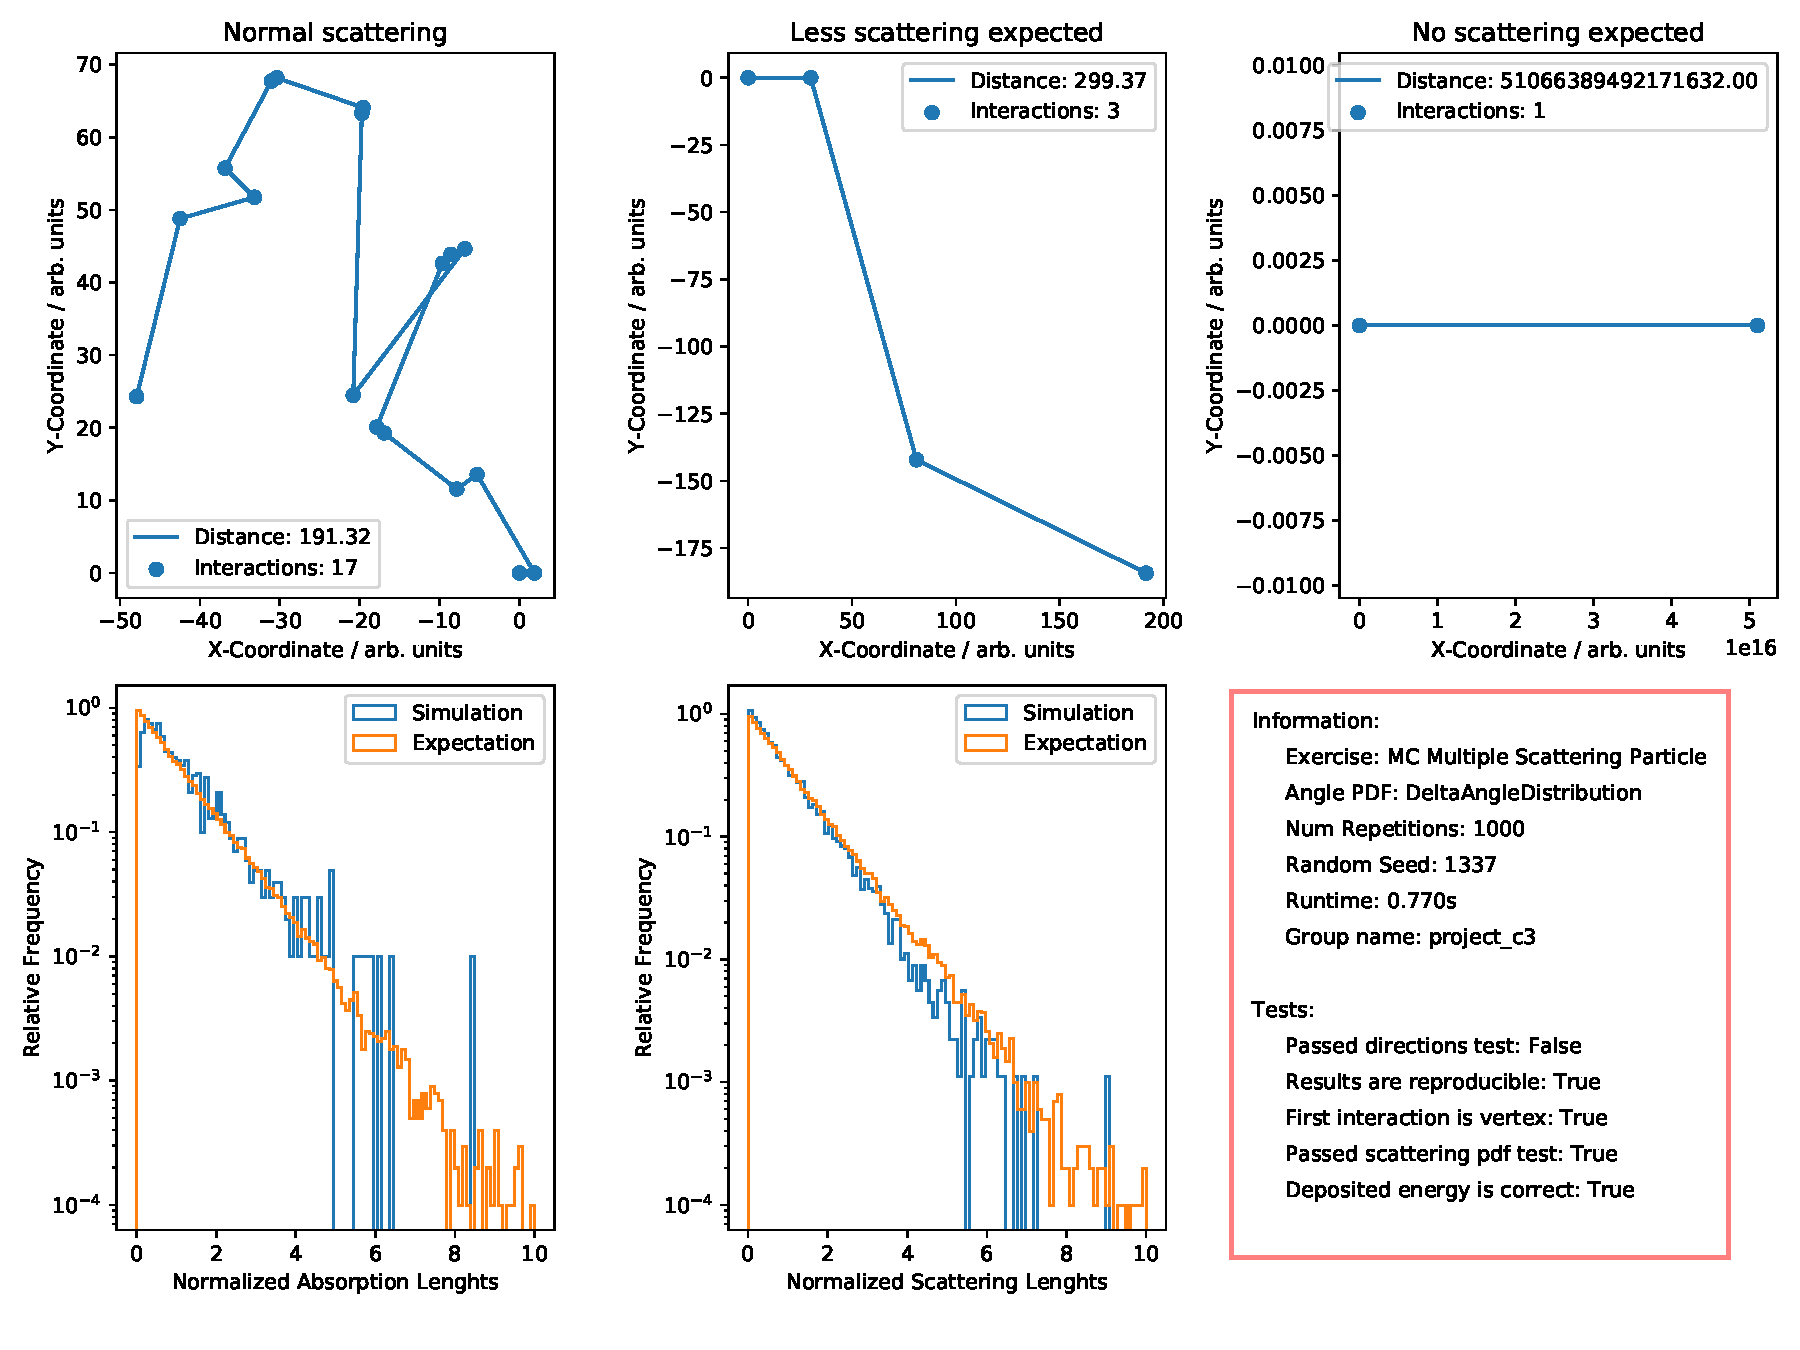
\includegraphics[width=\textwidth]{exercise_mc_multiple_scattering.pdf}

	\caption{Ergebnis der Testdatei von Aufgabe 2}

\end{figure}

Die graphischen Ergebisse stimmen mit der Erwartung überein. 
Lediglich der "Passed directions" Test wird als False ausgegenen.
Einen Fehler in der Implementierung oder bei den Ergebissen haben wir aber nicht gefunden.



\end{document}
